\documentclass[addpoints]{exam}
\usepackage{amsmath, amsfonts}
\usepackage{geometry}
\usepackage{hyperref}
\usepackage{titling}
\usepackage{tikz}
\usetikzlibrary{automata, positioning, arrows}


% Header and footer.
\pagestyle{headandfoot}
\runningheadrule
\runningfootrule
\runningheader{CS 212, Fall 2022}{HW 1: Regular Languages}{\theauthor}
\runningfooter{}{Page \thepage\ of \numpages}{}
\firstpageheader{}{}{}

\boxedpoints


\title{Homework 1: Regular Languages--Automata and Expressions}
    \author{pumping-string} % <=== replace with your team name
\date{CS 212 Nature of Computation\\Habib University\\Fall 2022}

\printanswers
\begin{document}

\maketitle

\begin{questions}

\question For each of the languages specified below, provide the formal specification and the state diagram of a finite automaton that recognizes it. 
  \begin{parts}
  \part[5] $L= \{w\in \{0,1\}^* \mid n_0(w)=2, n_1(w)\leq 5 \}$   where $n_x(w)$ denotes the count of $x$s in $w$.
  \begin{solution}
 The number of 0s in the language should be equal to 2, and the number of 1s should be less than or equal to 5.\\
 $L=\{00, 010, 100, 001, 1100, 0011, 1001, 0110, 11100...\}$
 \\the number of 0s should exactly 2 and number of 1s can be less than or equal to 5.
 \\number of $1s=0 , L= \{00\}$
 \\number of $1s= 1 , L= \{010, 100, 001\}$\\
 \begin{center}
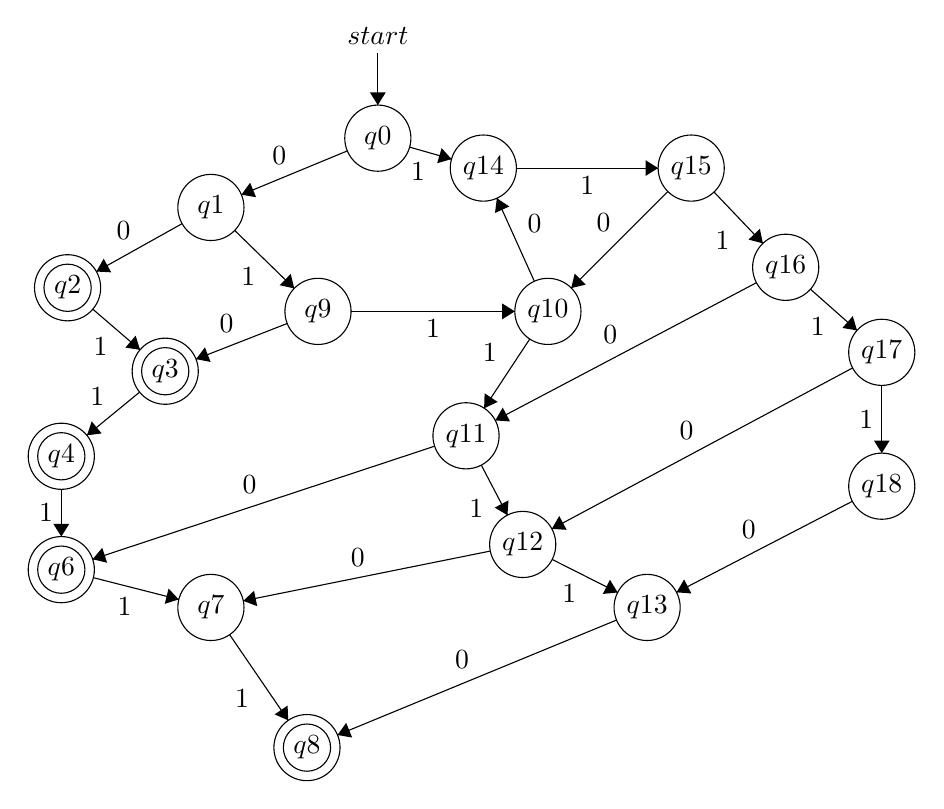
\begin{tikzpicture}[scale=0.2]
\tikzstyle{every node}+=[inner sep=0pt]
\draw [black] (22.5,-7.6) circle (2.1);
\draw (22.5,-7.6) node {$q0$};
\draw [black] (11.9,-12) circle (2.1);
\draw (11.9,-12) node {$q1$};
\draw [black] (2.8,-17.1) circle (2.1);
\draw (2.8,-17.1) node {$q2$};
\draw [black] (2.8,-17.1) circle (1.5);
\draw [black] (9,-22.4) circle (2.1);
\draw (9,-22.4) node {$q3$};
\draw [black] (9,-22.4) circle (1.5);
\draw [black] (2.4,-27.8) circle (2.1);
\draw (2.4,-27.8) node {$q4$};
\draw [black] (2.4,-27.8) circle (1.5);
\draw [black] (2.4,-35) circle (2.1);
\draw (2.4,-35) node {$q6$};
\draw [black] (2.4,-35) circle (1.5);
\draw [black] (11.9,-37.4) circle (2.1);
\draw (11.9,-37.4) node {$q7$};
\draw [black] (18,-46.3) circle (2.1);
\draw (18,-46.3) node {$q8$};
\draw [black] (18,-46.3) circle (1.5);
\draw [black] (18.7,-18.6) circle (2.1);
\draw (18.7,-18.6) node {$q9$};
\draw [black] (33.3,-18.6) circle (2.1);
\draw (33.3,-18.6) node {$q10$};
\draw [black] (28.1,-26.5) circle (2.1);
\draw (28.1,-26.5) node {$q11$};
\draw [black] (31.7,-33.4) circle (2.1);
\draw (31.7,-33.4) node {$q12$};
\draw [black] (39.6,-37.4) circle (2.1);
\draw (39.6,-37.4) node {$q13$};
\draw [black] (42.4,-9.5) circle (2.1);
\draw (42.4,-9.5) node {$q15$};
\draw [black] (48.4,-15.8) circle (2.1);
\draw (48.4,-15.8) node {$q16$};
\draw [black] (54.5,-21.2) circle (2.1);
\draw (54.5,-21.2) node {$q17$};
\draw [black] (54.5,-29.7) circle (2.1);
\draw (54.5,-29.7) node {$q18$};
\draw [black] (29.2,-9.5) circle (2.1);
\draw (29.2,-9.5) node {$q14$};
\draw [black] (22.5,-2.2) -- (22.5,-5.5);
\draw (22.5,-1.7) node [above] {$start$};
\fill [black] (22.5,-5.5) -- (23,-4.7) -- (22,-4.7);
\draw [black] (20.56,-8.41) -- (13.84,-11.19);
\fill [black] (13.84,-11.19) -- (14.77,-11.35) -- (14.39,-10.43);
\draw (16.24,-9.29) node [above] {$0$};
\draw [black] (10.07,-13.03) -- (4.63,-16.07);
\fill [black] (4.63,-16.07) -- (5.57,-16.12) -- (5.09,-15.25);
\draw (6.35,-14.05) node [above] {$0$};
\draw [black] (4.4,-18.46) -- (7.4,-21.04);
\fill [black] (7.4,-21.04) -- (7.12,-20.14) -- (6.47,-20.9);
\draw (4.89,-20.24) node [below] {$1$};
\draw [black] (7.37,-23.73) -- (4.03,-26.47);
\fill [black] (4.03,-26.47) -- (4.96,-26.35) -- (4.33,-25.58);
\draw (4.69,-24.61) node [above] {$1$};
\draw [black] (2.4,-29.9) -- (2.4,-32.9);
\fill [black] (2.4,-32.9) -- (2.9,-32.1) -- (1.9,-32.1);
\draw (1.9,-31.4) node [left] {$1$};
\draw [black] (4.44,-35.51) -- (9.86,-36.89);
\fill [black] (9.86,-36.89) -- (9.21,-36.2) -- (8.97,-37.17);
\draw (6.42,-36.77) node [below] {$1$};
\draw [black] (13.09,-39.13) -- (16.81,-44.57);
\fill [black] (16.81,-44.57) -- (16.77,-43.63) -- (15.95,-44.19);
\draw (14.35,-43.2) node [left] {$1$};
\draw [black] (13.41,-13.46) -- (17.19,-17.14);
\fill [black] (17.19,-17.14) -- (16.97,-16.22) -- (16.27,-16.94);
\draw (14.28,-15.78) node [below] {$1$};
\draw [black] (16.74,-19.37) -- (10.96,-21.63);
\fill [black] (10.96,-21.63) -- (11.88,-21.81) -- (11.52,-20.88);
\draw (12.9,-19.98) node [above] {$0$};
\draw [black] (24.52,-8.17) -- (27.18,-8.93);
\fill [black] (27.18,-8.93) -- (26.55,-8.23) -- (26.27,-9.19);
\draw (25.05,-9.11) node [below] {$1$};
\draw [black] (31.3,-9.5) -- (40.3,-9.5);
\fill [black] (40.3,-9.5) -- (39.5,-9) -- (39.5,-10);
\draw (35.8,-10) node [below] {$1$};
\draw [black] (43.85,-11.02) -- (46.95,-14.28);
\fill [black] (46.95,-14.28) -- (46.76,-13.36) -- (46.04,-14.04);
\draw (44.87,-14.12) node [left] {$1$};
\draw [black] (49.97,-17.19) -- (52.93,-19.81);
\fill [black] (52.93,-19.81) -- (52.66,-18.9) -- (52,-19.65);
\draw (50.44,-18.99) node [below] {$1$};
\draw [black] (54.5,-23.3) -- (54.5,-27.6);
\fill [black] (54.5,-27.6) -- (55,-26.8) -- (54,-26.8);
\draw (54,-25.45) node [left] {$1$};
\draw [black] (52.63,-30.66) -- (41.47,-36.44);
\fill [black] (41.47,-36.44) -- (42.41,-36.51) -- (41.95,-35.62);
\draw (46.06,-33.05) node [above] {$0$};
\draw [black] (52.65,-22.19) -- (33.55,-32.41);
\fill [black] (33.55,-32.41) -- (34.49,-32.47) -- (34.02,-31.59);
\draw (42.1,-26.8) node [above] {$0$};
\draw [black] (46.54,-16.78) -- (29.96,-25.52);
\fill [black] (29.96,-25.52) -- (30.9,-25.59) -- (30.43,-24.71);
\draw (37.26,-20.65) node [above] {$0$};
\draw [black] (40.92,-10.98) -- (34.78,-17.12);
\fill [black] (34.78,-17.12) -- (35.7,-16.9) -- (35,-16.2);
\draw (36.83,-13.57) node [above] {$0$};
\draw [black] (37.66,-38.2) -- (19.94,-45.5);
\fill [black] (19.94,-45.5) -- (20.87,-45.66) -- (20.49,-44.73);
\draw (27.84,-41.33) node [above] {$0$};
\draw [black] (29.64,-33.82) -- (13.96,-36.98);
\fill [black] (13.96,-36.98) -- (14.84,-37.32) -- (14.64,-36.34);
\draw (21.23,-34.81) node [above] {$0$};
\draw [black] (26.11,-27.16) -- (4.39,-34.34);
\fill [black] (4.39,-34.34) -- (5.31,-34.56) -- (5,-33.61);
\draw (14.36,-30.21) node [above] {$0$};
\draw [black] (20.8,-18.6) -- (31.2,-18.6);
\fill [black] (31.2,-18.6) -- (30.4,-18.1) -- (30.4,-19.1);
\draw (26,-19.1) node [below] {$1$};
\draw [black] (32.15,-20.35) -- (29.25,-24.75);
\fill [black] (29.25,-24.75) -- (30.11,-24.35) -- (29.28,-23.8);
\draw (30.09,-21.22) node [left] {$1$};
\draw [black] (29.07,-28.36) -- (30.73,-31.54);
\fill [black] (30.73,-31.54) -- (30.8,-30.6) -- (29.92,-31.06);
\draw (29.22,-31.1) node [left] {$1$};
\draw [black] (33.57,-34.35) -- (37.73,-36.45);
\fill [black] (37.73,-36.45) -- (37.24,-35.64) -- (36.79,-36.54);
\draw (34.66,-35.9) node [below] {$1$};
\draw [black] (32.44,-16.69) -- (30.06,-11.41);
\fill [black] (30.06,-11.41) -- (29.94,-12.35) -- (30.85,-11.94);
\draw (31.97,-13.04) node [right] {$0$};
\end{tikzpicture}
\end{center}

 
  \end{solution}
  
  \part[5] $(((00)^*(11))\cup 01)^*$.\\\
  \begin{solution}
  $(00)^*$
  \begin{center}
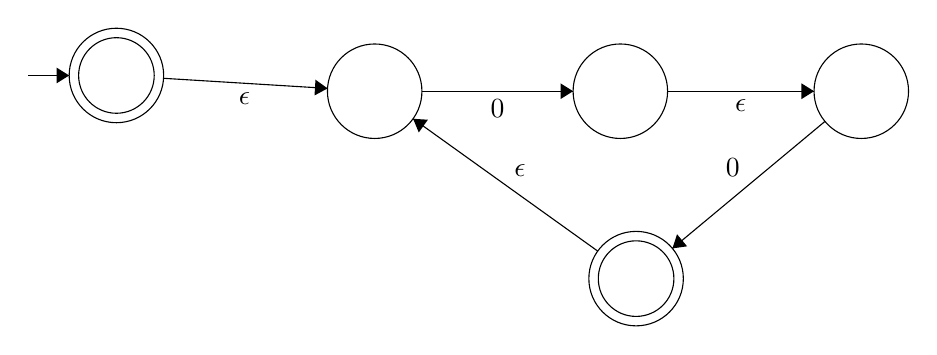
\begin{tikzpicture}[scale=0.2]
\tikzstyle{every node}+=[inner sep=0pt]
\draw [black] (22.2,-4.2) circle (3);
\draw [black] (37.8,-4.2) circle (3);
\draw [black] (53.1,-4.2) circle (3);
\draw [black] (38.8,-16.1) circle (3);
\draw [black] (38.8,-16.1) circle (2.4);
\draw [black] (5.8,-3.2) circle (3);
\draw [black] (5.8,-3.2) circle (2.4);
\draw [black] (25.2,-4.2) -- (34.8,-4.2);
\fill [black] (34.8,-4.2) -- (34,-3.7) -- (34,-4.7);
\draw (30,-4.7) node [below] {$0$};
\draw [black] (40.8,-4.2) -- (50.1,-4.2);
\fill [black] (50.1,-4.2) -- (49.3,-3.7) -- (49.3,-4.7);
\draw (45.45,-4.7) node [below] {$\epsilon$};
\draw [black] (50.79,-6.12) -- (41.11,-14.18);
\fill [black] (41.11,-14.18) -- (42.04,-14.05) -- (41.4,-13.28);
\draw (44.94,-9.66) node [above] {$0$};
\draw [black] (0.2,-3.2) -- (2.8,-3.2);
\fill [black] (2.8,-3.2) -- (2,-2.7) -- (2,-3.7);
\draw [black] (36.36,-14.35) -- (24.64,-5.95);
\fill [black] (24.64,-5.95) -- (25,-6.82) -- (25.58,-6.01);
\draw (31.42,-9.65) node [above] {$\epsilon$};
\draw [black] (8.79,-3.38) -- (19.21,-4.02);
\fill [black] (19.21,-4.02) -- (18.44,-3.47) -- (18.38,-4.47);
\draw (13.93,-4.25) node [below] {$\epsilon$};
\end{tikzpicture}
\end{center}
$(11)$\\
\begin{center}
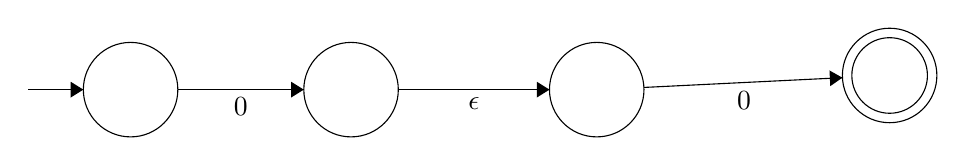
\begin{tikzpicture}[scale=0.2]
\tikzstyle{every node}+=[inner sep=0pt]
\draw [black] (20.7,-4.1) circle (3);
\draw [black] (36.3,-4.1) circle (3);
\draw [black] (6.7,-4.1) circle (3);
\draw [black] (54.9,-3.2) circle (3);
\draw [black] (54.9,-3.2) circle (2.4);
\draw [black] (23.7,-4.1) -- (33.3,-4.1);
\fill [black] (33.3,-4.1) -- (32.5,-3.6) -- (32.5,-4.6);
\draw (28.5,-4.6) node [below] {$\epsilon$};
\draw [black] (39.3,-3.96) -- (51.9,-3.34);
\fill [black] (51.9,-3.34) -- (51.08,-2.88) -- (51.13,-3.88);
\draw (45.65,-4.2) node [below] {$0$};
\draw [black] (9.7,-4.1) -- (17.7,-4.1);
\fill [black] (17.7,-4.1) -- (16.9,-3.6) -- (16.9,-4.6);
\draw (13.7,-4.6) node [below] {$0$};
\draw [black] (0.2,-4.1) -- (3.7,-4.1);
\fill [black] (3.7,-4.1) -- (2.9,-3.6) -- (2.9,-4.6);
\end{tikzpicture}
\end{center}
$(00)^*(11)$\\
\begin{center}
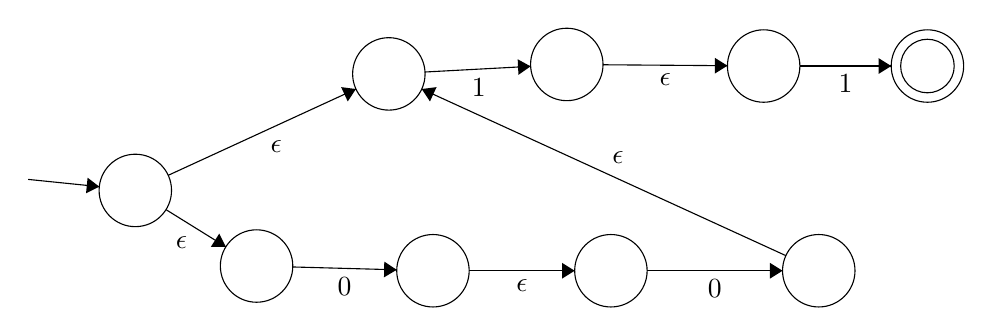
\begin{tikzpicture}[scale=0.2]
\tikzstyle{every node}+=[inner sep=0pt]
\draw [black] (7,-10.5) circle (2.3);
\draw [black] (14.7,-15.3) circle (2.3);
\draw [black] (25.9,-15.6) circle (2.3);
\draw [black] (37.2,-15.6) circle (2.3);
\draw [black] (50.4,-15.6) circle (2.3);
\draw [black] (23.1,-3.1) circle (2.3);
\draw [black] (34.4,-2.5) circle (2.3);
\draw [black] (46.9,-2.6) circle (2.3);
\draw [black] (57.3,-2.6) circle (2.3);
\draw [black] (57.3,-2.6) circle (1.7);
\draw [black] (49.2,-2.6) -- (55,-2.6);
\fill [black] (55,-2.6) -- (54.2,-2.1) -- (54.2,-3.1);
\draw (52.1,-3.1) node [below] {$1$};
\draw [black] (36.7,-2.52) -- (44.6,-2.58);
\fill [black] (44.6,-2.58) -- (43.8,-2.08) -- (43.8,-3.08);
\draw (40.65,-3.06) node [below] {$\epsilon$};
\draw [black] (25.4,-2.98) -- (32.1,-2.62);
\fill [black] (32.1,-2.62) -- (31.28,-2.17) -- (31.33,-3.16);
\draw (28.81,-3.35) node [below] {$1$};
\draw [black] (9.09,-9.54) -- (21.01,-4.06);
\fill [black] (21.01,-4.06) -- (20.07,-3.94) -- (20.49,-4.85);
\draw (15.95,-7.31) node [below] {$\epsilon$};
\draw [black] (8.95,-11.72) -- (12.75,-14.08);
\fill [black] (12.75,-14.08) -- (12.33,-13.24) -- (11.8,-14.08);
\draw (9.93,-13.4) node [below] {$\epsilon$};
\draw [black] (17,-15.36) -- (23.6,-15.54);
\fill [black] (23.6,-15.54) -- (22.81,-15.02) -- (22.79,-16.02);
\draw (20.29,-15.98) node [below] {$0$};
\draw [black] (28.2,-15.6) -- (34.9,-15.6);
\fill [black] (34.9,-15.6) -- (34.1,-15.1) -- (34.1,-16.1);
\draw (31.55,-16.1) node [below] {$\epsilon$};
\draw [black] (39.5,-15.6) -- (48.1,-15.6);
\fill [black] (48.1,-15.6) -- (47.3,-15.1) -- (47.3,-16.1);
\draw (43.8,-16.1) node [below] {$0$};
\draw [black] (48.31,-14.64) -- (25.19,-4.06);
\fill [black] (25.19,-4.06) -- (25.71,-4.85) -- (26.13,-3.94);
\draw (37.65,-8.84) node [above] {$\epsilon$};
\draw [black] (0.2,-9.8) -- (4.71,-10.26);
\fill [black] (4.71,-10.26) -- (3.97,-9.69) -- (3.87,-10.68);
\end{tikzpicture}
\end{center}
$(00)^*(11) \cup (11)$
\\
\begin{center}
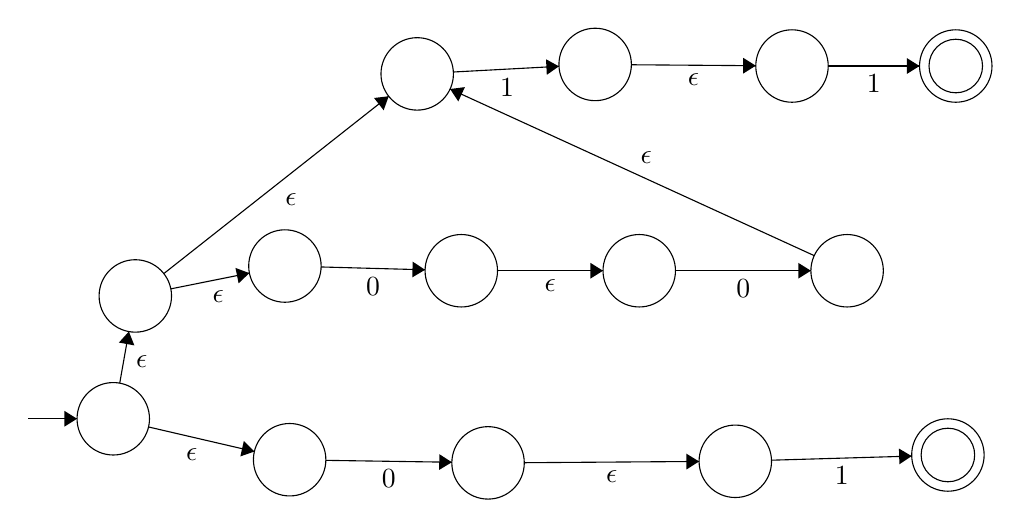
\begin{tikzpicture}[scale=0.2]
\tikzstyle{every node}+=[inner sep=0pt]
\draw [black] (7,-17.2) circle (2.3);
\draw [black] (16.5,-15.3) circle (2.3);
\draw [black] (27.7,-15.6) circle (2.3);
\draw [black] (39,-15.6) circle (2.3);
\draw [black] (52.2,-15.6) circle (2.3);
\draw [black] (24.9,-3.1) circle (2.3);
\draw [black] (36.2,-2.5) circle (2.3);
\draw [black] (48.7,-2.6) circle (2.3);
\draw [black] (59.1,-2.6) circle (2.3);
\draw [black] (59.1,-2.6) circle (1.7);
\draw [black] (5.6,-25) circle (2.3);
\draw [black] (16.8,-27.6) circle (2.3);
\draw [black] (29.4,-27.8) circle (2.3);
\draw [black] (45.1,-27.7) circle (2.3);
\draw [black] (58.6,-27.3) circle (2.3);
\draw [black] (58.6,-27.3) circle (1.7);
\draw [black] (51,-2.6) -- (56.8,-2.6);
\fill [black] (56.8,-2.6) -- (56,-2.1) -- (56,-3.1);
\draw (53.9,-3.1) node [below] {$1$};
\draw [black] (38.5,-2.52) -- (46.4,-2.58);
\fill [black] (46.4,-2.58) -- (45.6,-2.08) -- (45.6,-3.08);
\draw (42.45,-3.06) node [below] {$\epsilon$};
\draw [black] (27.2,-2.98) -- (33.9,-2.62);
\fill [black] (33.9,-2.62) -- (33.08,-2.17) -- (33.13,-3.16);
\draw (30.61,-3.35) node [below] {$1$};
\draw [black] (8.81,-15.78) -- (23.09,-4.52);
\fill [black] (23.09,-4.52) -- (22.16,-4.63) -- (22.77,-5.41);
\draw (16.88,-10.65) node [below] {$\epsilon$};
\draw [black] (9.26,-16.75) -- (14.24,-15.75);
\fill [black] (14.24,-15.75) -- (13.36,-15.42) -- (13.56,-16.4);
\draw (12.27,-16.83) node [below] {$\epsilon$};
\draw [black] (18.8,-15.36) -- (25.4,-15.54);
\fill [black] (25.4,-15.54) -- (24.61,-15.02) -- (24.59,-16.02);
\draw (22.09,-15.98) node [below] {$0$};
\draw [black] (30,-15.6) -- (36.7,-15.6);
\fill [black] (36.7,-15.6) -- (35.9,-15.1) -- (35.9,-16.1);
\draw (33.35,-16.1) node [below] {$\epsilon$};
\draw [black] (41.3,-15.6) -- (49.9,-15.6);
\fill [black] (49.9,-15.6) -- (49.1,-15.1) -- (49.1,-16.1);
\draw (45.6,-16.1) node [below] {$0$};
\draw [black] (50.11,-14.64) -- (26.99,-4.06);
\fill [black] (26.99,-4.06) -- (27.51,-4.85) -- (27.93,-3.94);
\draw (39.45,-8.84) node [above] {$\epsilon$};
\draw [black] (0.2,-25) -- (3.3,-25);
\fill [black] (3.3,-25) -- (2.5,-24.5) -- (2.5,-25.5);
\draw [black] (6.01,-22.74) -- (6.59,-19.46);
\fill [black] (6.59,-19.46) -- (5.96,-20.16) -- (6.94,-20.34);
\draw (7.02,-21.36) node [right] {$\epsilon$};
\draw [black] (47.4,-27.63) -- (56.3,-27.37);
\fill [black] (56.3,-27.37) -- (55.49,-26.89) -- (55.52,-27.89);
\draw (51.87,-28.03) node [below] {$1$};
\draw [black] (31.7,-27.79) -- (42.8,-27.71);
\fill [black] (42.8,-27.71) -- (42,-27.22) -- (42,-28.22);
\draw (37.25,-28.26) node [below] {$\epsilon$};
\draw [black] (19.1,-27.64) -- (27.1,-27.76);
\fill [black] (27.1,-27.76) -- (26.31,-27.25) -- (26.29,-28.25);
\draw (23.09,-28.22) node [below] {$0$};
\draw [black] (7.84,-25.52) -- (14.56,-27.08);
\fill [black] (14.56,-27.08) -- (13.89,-26.41) -- (13.67,-27.39);
\draw (10.59,-26.87) node [below] {$\epsilon$};
\end{tikzpicture}
\end{center}
$((00)^*(11) \cup (11))^*$\\


\begin{center}
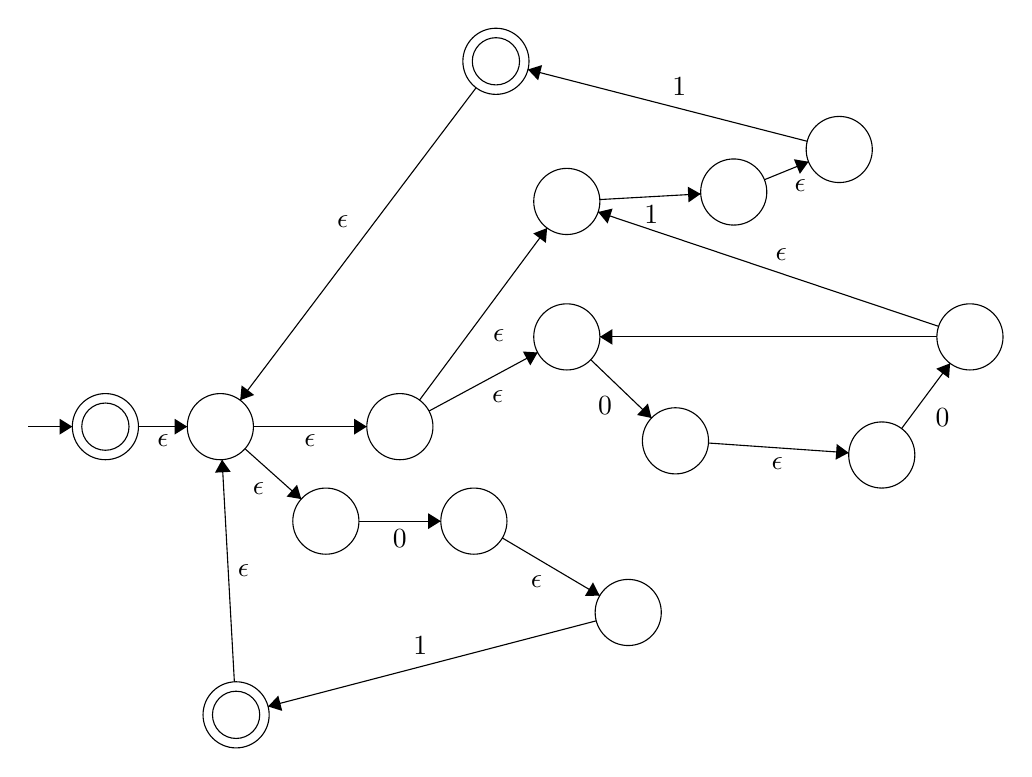
\begin{tikzpicture}[scale=0.2]
\tikzstyle{every node}+=[inner sep=0pt]
\draw [black] (34.4,-11) circle (2.1);
\draw [black] (45,-10.4) circle (2.1);
\draw [black] (51.7,-7.7) circle (2.1);
\draw [black] (29.9,-2.1) circle (2.1);
\draw [black] (29.9,-2.1) circle (1.5);
\draw [black] (23.8,-25.3) circle (2.1);
\draw [black] (34.4,-19.6) circle (2.1);
\draw [black] (41.3,-26.2) circle (2.1);
\draw [black] (54.4,-27.1) circle (2.1);
\draw [black] (60,-19.6) circle (2.1);
\draw [black] (13.4,-43.6) circle (2.1);
\draw [black] (13.4,-43.6) circle (1.5);
\draw [black] (38.3,-37.1) circle (2.1);
\draw [black] (28.5,-31.3) circle (2.1);
\draw [black] (19.1,-31.3) circle (2.1);
\draw [black] (12.4,-25.3) circle (2.1);
\draw [black] (5.1,-25.3) circle (2.1);
\draw [black] (5.1,-25.3) circle (1.5);
\draw [black] (0.2,-25.3) -- (3,-25.3);
\fill [black] (3,-25.3) -- (2.2,-24.8) -- (2.2,-25.8);
\draw [black] (7.2,-25.3) -- (10.3,-25.3);
\fill [black] (10.3,-25.3) -- (9.5,-24.8) -- (9.5,-25.8);
\draw (8.75,-25.8) node [below] {$\epsilon$};
\draw [black] (14.5,-25.3) -- (21.7,-25.3);
\fill [black] (21.7,-25.3) -- (20.9,-24.8) -- (20.9,-25.8);
\draw (18.1,-25.8) node [below] {$\epsilon$};
\draw [black] (25.65,-24.31) -- (32.55,-20.59);
\fill [black] (32.55,-20.59) -- (31.61,-20.53) -- (32.08,-21.41);
\draw (30.02,-22.95) node [below] {$\epsilon$};
\draw [black] (35.92,-21.05) -- (39.78,-24.75);
\fill [black] (39.78,-24.75) -- (39.55,-23.83) -- (38.86,-24.56);
\draw (36.83,-23.38) node [below] {$0$};
\draw [black] (43.4,-26.34) -- (52.3,-26.96);
\fill [black] (52.3,-26.96) -- (51.54,-26.4) -- (51.47,-27.4);
\draw (47.76,-27.21) node [below] {$\epsilon$};
\draw [black] (55.66,-25.42) -- (58.74,-21.28);
\fill [black] (58.74,-21.28) -- (57.86,-21.62) -- (58.67,-22.22);
\draw (57.78,-24.74) node [right] {$0$};
\draw [black] (58.01,-18.93) -- (36.39,-11.67);
\fill [black] (36.39,-11.67) -- (36.99,-12.4) -- (37.31,-11.45);
\draw (48.02,-14.77) node [above] {$\epsilon$};
\draw [black] (36.5,-10.88) -- (42.9,-10.52);
\fill [black] (42.9,-10.52) -- (42.08,-10.06) -- (42.13,-11.06);
\draw (39.76,-11.25) node [below] {$1$};
\draw [black] (46.95,-9.62) -- (49.75,-8.48);
\fill [black] (49.75,-8.48) -- (48.82,-8.32) -- (49.2,-9.25);
\draw (49.23,-9.57) node [below] {$\epsilon$};
\draw [black] (49.67,-7.18) -- (31.93,-2.62);
\fill [black] (31.93,-2.62) -- (32.58,-3.31) -- (32.83,-2.34);
\draw (41.54,-4.33) node [above] {$1$};
\draw [black] (36.27,-37.63) -- (15.43,-43.07);
\fill [black] (15.43,-43.07) -- (16.33,-43.35) -- (16.08,-42.38);
\draw (25.1,-39.78) node [above] {$1$};
\draw [black] (30.31,-32.37) -- (36.49,-36.03);
\fill [black] (36.49,-36.03) -- (36.06,-35.19) -- (35.55,-36.05);
\draw (32.48,-34.7) node [below] {$\epsilon$};
\draw [black] (21.2,-31.3) -- (26.4,-31.3);
\fill [black] (26.4,-31.3) -- (25.6,-30.8) -- (25.6,-31.8);
\draw (23.8,-31.8) node [below] {$0$};
\draw [black] (13.96,-26.7) -- (17.54,-29.9);
\fill [black] (17.54,-29.9) -- (17.27,-28.99) -- (16.61,-29.74);
\draw (14.82,-28.79) node [below] {$\epsilon$};
\draw [black] (57.9,-19.6) -- (36.5,-19.6);
\fill [black] (36.5,-19.6) -- (37.3,-20.1) -- (37.3,-19.1);
\draw [black] (13.29,-41.5) -- (12.51,-27.4);
\fill [black] (12.51,-27.4) -- (12.06,-28.22) -- (13.06,-28.17);
\draw (13.48,-34.42) node [right] {$\epsilon$};
\draw [black] (28.64,-3.78) -- (13.66,-23.62);
\fill [black] (13.66,-23.62) -- (14.55,-23.29) -- (13.75,-22.68);
\draw (20.57,-12.3) node [left] {$\epsilon$};
\draw [black] (25.05,-23.61) -- (33.15,-12.69);
\fill [black] (33.15,-12.69) -- (32.27,-13.03) -- (33.07,-13.63);
\draw (29.68,-19.54) node [right] {$\epsilon$};
\end{tikzpicture}
\end{center}




  
  
  
  \end{solution}
    
  \end{parts}
  

  Please see \href{https://www3.nd.edu/~kogge/courses/cse30151-fa17/Public/other/tikz_tutorial.pdf}{this guide} for help on drawing state diagrams.
  
\question[5] Below is the transition table of a finite automaton. $\implies$ indicates the starting state, and $*$ indicates accepting states. Provide a regular expression for the language recognized by this automaton.
  \[
  \begin{array}{r|cc}
    & 0 & 1 \\\hline
    p & \{ q \} & \emptyset \\
    \implies q & \{ q \} & \{ q, r \} \\
    *r & \emptyset & \{ s \} \\
    *s & \emptyset & \emptyset \\
  \end{array}
  \]
  \begin{solution}
  \begin{center}
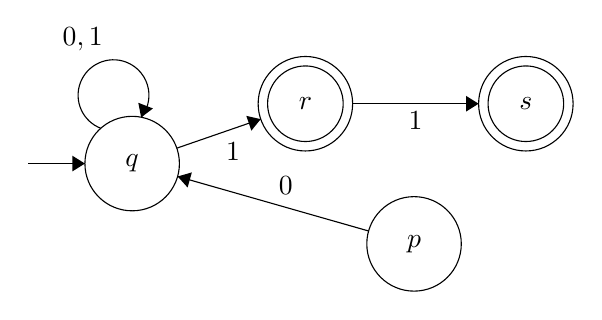
\begin{tikzpicture}[scale=0.2]
\tikzstyle{every node}+=[inner sep=0pt]
\draw [black] (6.8,-8.9) circle (3);
\draw (6.8,-8.9) node {$q$};
\draw [black] (17.8,-5.1) circle (3);
\draw (17.8,-5.1) node {$r$};
\draw [black] (17.8,-5.1) circle (2.4);
\draw [black] (31.8,-5.1) circle (3);
\draw (31.8,-5.1) node {$s$};
\draw [black] (31.8,-5.1) circle (2.4);
\draw [black] (24.7,-14) circle (3);
\draw (24.7,-14) node {$p$};
\draw [black] (9.64,-7.92) -- (14.96,-6.08);
\fill [black] (14.96,-6.08) -- (14.05,-5.87) -- (14.37,-6.81);
\draw (13.21,-7.53) node [below] {$1$};
\draw [black] (20.8,-5.1) -- (28.8,-5.1);
\fill [black] (28.8,-5.1) -- (28,-4.6) -- (28,-5.6);
\draw (24.8,-5.6) node [below] {$1$};
\draw [black] (21.81,-13.18) -- (9.69,-9.72);
\fill [black] (9.69,-9.72) -- (10.32,-10.42) -- (10.59,-9.46);
\draw (16.56,-10.89) node [above] {$0$};
\draw [black] (4.819,-6.663) arc (249.25512:-38.74488:2.25);
\draw (3.66,-1.78) node [above] {$0,1$};
\fill [black] (7.37,-5.97) -- (8.12,-5.4) -- (7.19,-5.04);
\draw [black] (0.2,-8.9) -- (3.8,-8.9);
\fill [black] (3.8,-8.9) -- (3,-8.4) -- (3,-9.4);
\end{tikzpicture}
\end{center}
The Regular Expression for this finite automate will be
\begin{center}
    $(0 \cup 1)^*1$
\end{center}
 

  \end{solution}
  
\question
  \begin{parts}
  \part[5] Suggest regular languages $L_1$ and $L_2$ over $\{0,1\}$ such that
  \begin{enumerate}
  \item $L_1\not\subseteq L_2$,
  \item $L_2\not\subseteq L_1$, and
  \item $(L_1\cup L_2)^* = L_1^* \cup L_2^*$
  \end{enumerate}
  \begin{solution}suggestion:\\
  if we take $L_1$ such that
  $L_1= \{w \mid \{ 0\} \}$ \\
  if we take $L_2$ such that
  $L_2= \{w \mid \{ \epsilon\} \}$(empty string) \\
  condition 1 and 2 will be satisfied easily as $\{0\}$ is not a subset of $\{ \epsilon \}$ and vice versa.\\
  to satisfy condition 3 we break the condition into the left side and the right side.\\
  left side $(L_1\cup L_2)^*$ will be $(0\cup \epsilon )^*$ resulting in the set $\{ \epsilon,0,00,000,0000... \}$\\
  right side $L_1^* \cup L_2^*$ will be $0^* \cup \epsilon^* = (0 \cup \epsilon),(00 \cup \epsilon), (000 \cup \epsilon)...$ and so on. this also results in the set  $\{ \epsilon,0,00,000,0000... \}$\\
  with that we can say that our suggestion for $L_1$ and $L_2$ holds and $(L_1\cup L_2)^* = L_1^* \cup L_2^*$
  
  
  
  \end{solution}
  \part[5] Prove or disprove whether condition 3 above holds for any regular languages, $L_1$ and $L_2$.
  \begin{solution}
  to disprove:\\
  suppose we take $L_1= \{w \mid \{1\} \}$ and $L_2= \{w \mid \{0\} \}$
  then:\\
  $(L_1\cup L_2)^* = L_1^* \cup L_2^*$ will be\\
   left side is $(L_1\cup L_2)^* = \{ \epsilon ,0,1,01,10,0010,01100,100...\}$\\
  right side is $L_1^* \cup L_2^* = \{ \epsilon,0,1,01,01,11,00,0011...\}$\\ 
  $(L_1\cup L_2)^*$ can allow 0's and 1's to be located anywhere in the string\\
  while $L_1^* \cup L_2^*$ will have all the 0's on the left and all the 1's towards the right\\
  we can conclude that these 2 languages do not satisfy condition 3 \\
  hence $(L_1\cup L_2)^* \neq L_1^* \cup L_2^*$
  
  
  
  \end{solution}
  \end{parts}

\question[5] In class, we talked about the closure of the class, $A$, of regular languages under the union, concatenation, and star operations. In this question, we want to explore whether $A$ is also closed under intersection. That is, does the following hold?
  \[
    L_1\in A \land L_2\in A \implies L_1 \cap L_2\in A
  \]

  We want to go about it as follows. The expression, $L_1 \cap L_2$, can be transformed using DeMorgan's law to an equivalent one involving union, for which closure is known, and another operation. Show whether $A$ is closed under this operation, and use your result to argue about the closure of $A$ under intersection.
  \begin{solution}
 \[ L_1\in A \land L_2\in A \implies L_1 \cap L_2\in A \]
  1. Assuming that the languages $L_1$ and $L_2$ are regular languages and belong to the regular language $A$.
  Using LHS,
  $L_1 \cap L_2\in A$, can also be written as: $L_1 \in A \cap L_2\in A$
 \\
  2. Using De morgan's law, the expression $L_1 \cap L_2$ can be transformed into union and complement operation. 
  $L_1 \cap L_2 = \overline{\overline{L_1}\cup  \overline{L_2}} $
  \\
  3. Let $Q = (Q,\epsilon,\sigma, q_0,F)$be a DFA that accepts $L_1$. Then, $Q =(Q,\epsilon,\sigma,q_0,F)$ accepts $\overline{L_1}$. This is because if we switch the final and non final states of the existing DFA then the new DFA accepts the language $\overline{L_1}$. Now, Language $\overline{L_1}$ is also a regular language, so there exists a DFA that the accepts the complement of the language. Hence, a set of regular language is closed under complement operation. Since, regular languages are closed under complement operation we can say that languages $\overline{L_1}$ and  $\overline{L_2}$ are also regular, so $\overline{L_1} \in A$ and $\overline{L_2} \in A$.
  \\
  4.Similarly, the set of regular languages A is closed under union operation. Therefore, ${\overline{L_1}\cup  \overline{L_2}} $ are also regular languages, so  ${\overline{L_1}\cup  \overline{L_2}} \in A $. Subsequently, $\overline{\overline{L_1}\cup  \overline{L_2}} $ is also a part of regular language because the set of regular languages A is closed under complement operation. $\overline{\overline{L_1}\cup  \overline{L_2}}\in A $. Hence, the closure of A is also closed under intersection.
  \\

 
  
  
  
  
  \end{solution}

\question[5] We now want to explore the closure of the class, $A$, of regular languages under the operation, $mix$, which is defined as follows.
  \begin{itemize}
  \item Given strings, $u$ and $v$, both of length $n$, $mix(u,v) = u_1v_1u_2v_2\ldots u_nv_n$.
  \item Given languages, $L_1$ and $L_2$, $mix(L_1,L_2) = \{mix(u,v) \mid u\in L_1, v\in L_2, |u| = |v|\}$.
  \end{itemize}
  Is $A$ closed under $mix$? Justify your answer.
  \begin{solution}
  mix(u,v) has two strings u and v both of equal length n. the concatenation of strings u and v is returned by the operation mix. For example, if u="0011" and v= "1100", mix(u,v)= "00111100". 
  \\
  \\
  Given the languages $L_1$ and $L_2$, the operation mix($L_1$,$L_2$) will return the string formed by the concatenation of both the strings, $L_1$ and $L_2$. It will return a set of language that consists of all the possible strings that is formed by the concatenation of one string from $L_1$ to one string from $L_2$. If if $L_1=("0", "01", "011", "0111)$ and $L_2= "1" "10" "100", "1000"$, $mix(u,v)= ("01" "0110", "011100", "01111000")$. 
  \\\\
 Proof:
 To prove that a is closed under the mix, we can construct a regular language that is a mix of two regular languages. 
 $L_1 = (u,v)*$
 $L_2= (1,0)*$
 mix($L_1$,$L_2)= (u,v,1,0)*$. 
 Therefore, we can conclude that A is closed under the mix.
  \end{solution}
  
\end{questions}

\end{document}

%%% Local Variables:
%%% mode: latex
%%% TeX-master: t
%%% End:
